\documentclass{standalone}
\usepackage{pgfplots}
\pgfplotsset{compat=1.18}

\definecolor{myDarkGray}{gray}{0.3}  
\definecolor{myMidGray}{gray}{0.55}   
\definecolor{myLightGray}{gray}{0.75}  

\begin{document}
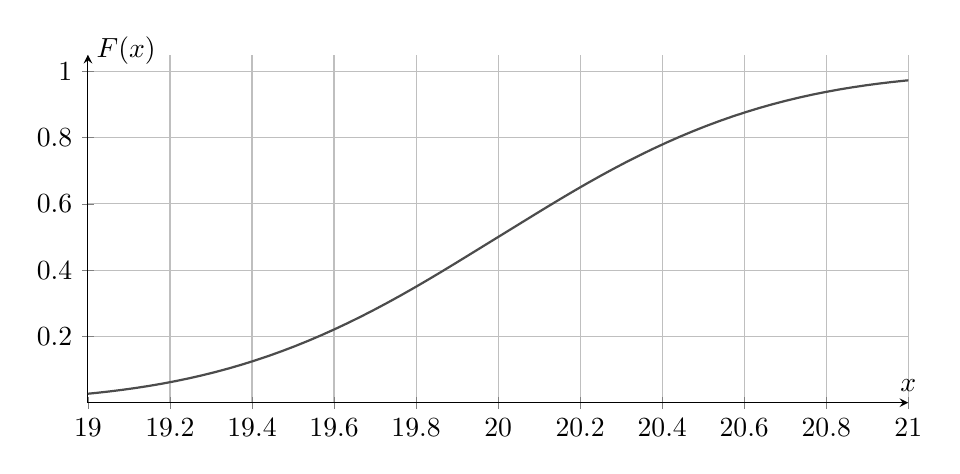
\begin{tikzpicture}
\pgfmathdeclarefunction{erf}{1}{%
  \pgfmathparse{sign(#1)*(1 - 1/(1 + 0.278393*abs(#1) + 0.230389*abs(#1)^2 + 0.000972*abs(#1)^3 + 0.078108*abs(#1)^4)^4)}%
}
\begin{axis}[
    xlabel={$x$},
    ylabel={$F(x)$},
    grid=major,
    width=12cm,
    height=6cm,
    ymin=0, ymax=1.05,
    ytick={0.2,0.4,...,1},
    xmin=19, xmax=21,
    xtick={19,19.2,...,21},
    axis lines=left,
    xlabel style={at={(ticklabel* cs:1)}, anchor=north, yshift=12pt},
    ylabel style={
        at={(ticklabel* cs:1)}, 
        anchor=north east,
        rotate=-90, 
        xshift=28pt,
        yshift=10pt}
]

% CDF der Standardnormalverteilung (mu=0, sigma=1)
% Formel: 0.5*(1 + erf(x / sqrt(2)))
\addplot [
    domain=18.6:21.8, 
    samples=100, 
    color=myDarkGray, 
    thick
] {0.5*(1 + erf((x-20)/(0.52*sqrt(2))))};

\end{axis}
\end{tikzpicture}
\end{document}